\chapter{Python\index{Python}}
\thispagestyle{fancy}
\lstset{}\lstset{language=Python, style=pythonstyle}

Python is a high-level, interpreted programming language known for its simplicity, readability, and versatility. With its elegant syntax and dynamic typing, Python facilitates rapid development and prototyping across various domains, including web development, data analysis, artificial intelligence, and scientific computing. Its extensive standard library and vibrant ecosystem of third-party packages provide comprehensive support for a wide range of tasks, from basic scripting to complex software development. Python's object-oriented and functional programming paradigms, coupled with its strong community support and cross-platform compatibility, make it an ideal choice for both beginners and experienced developers seeking efficient and expressive solutions to their programming challenges. Its emphasis on code readability and simplicity distinguishes Python from other languages, promoting maintainability and collaboration in software projects.

\myindent The official python documentation can be found at the following links
\begin{lstlisting}
# Documentation for version 3+
https://docs.python.org/3/
# Documentation for version 2+
https://docs.python.org/2/
\end{lstlisting}











\section{Basics of Python}












\subsection{Imports and libraries}

Import floating point division which allows python 2 compatibility when using division with doubles. Include this at the beginning of the script.
\begin{lstlisting}
from __future__ import division
\end{lstlisting}

On Linux, there's a site-packages folder that imported libraries are all in. These are located in the following directories for python versions 2.7 and 3.6 respectively.

\begin{itemize}
	\item /usr/lib/python2.7/site-packages
	\item /usr/lib/python3.6/site-packages
\end{itemize}

I believe you only have specify the path from that folder on. For example, an app that uses the import program.script.interface as interface will have the interface.py file installed to usr/lib/python3.6/site-packages/program/scripts.









\subsection{Program parameters}

You can add input parameters for a python script/program using the argparse package.
\begin{lstlisting}
import argparse

parser.add_argument(
		'-v',							# Creats a parameter with -v
		'--verbose',					# Creates args.verbose parameter
		required=False,					# Sets the parameter to not required.
		default=False,					# Sets default value
		action='store_true',			# Sets value to true if supplied
		help="Enables verbose mode.")	# Sets help message
					
parser.add_argument(
		'-i',							# Creates a parameter with -i
		'--input',						# Creates args.input parameter
		required=True,					# Sets the parameter to be required
		default="potato",				# Sets default value to "potato"
		help="An input string to use")	# Sets a help message
		
if args.input is not none:
	print("Input value is {0}".format(args.input)) # prints the input value.
	
if args.verbose:
	print("Verbose is on!")
\end{lstlisting}





\subsection{Methods, Functions, and Classes}


To define a \idx{function} in Python, you use the \idx{def} keyword followed by the function name and parameters, if any. You can also include a docstring to provide documentation for the function. In this example, the \texttt{greet()} function takes a \texttt{name} parameter and returns a greeting message.
\begin{lstlisting}
def greet(name):
    """
    This function greets the user.
    :param name: The name of the person to greet
    :return: A greeting message
    """
    return f"Hello, {name}!"
\end{lstlisting}


\idx{Methods} are functions that are associated with objects. They are defined within the scope of a class and are accessed through instances of the class. In this example, the \texttt{bark()} method of the \texttt{Dog} class prints a bark message when called.
\begin{lstlisting}
class Dog:
    def bark(self):
        """
        This method makes the dog bark.
        """
        print("Woof!")
\end{lstlisting}

\idx{Classes} in Python allow you to define your own data types with custom attributes and methods. In this example, the \texttt{Rectangle} class represents a geometric rectangle. It has an \idx{\_\_init\_\_()} method to initialize its width and height attributes and an \texttt{area()} method to calculate its area.
\begin{lstlisting}
class Rectangle:
    def __init__(self, width, height):
        self.width = width
        self.height = height
        
    def area(self):
        return self.width * self.height
\end{lstlisting}

To use the \texttt{Rectangle} class, you can create an instance of it by passing the width and height values as parameters to the constructor:
\begin{lstlisting}
# Constructing a Rectangle object
rectangle1 = Rectangle(5, 10)

# Calculating the area of the rectangle
area = rectangle1.area()

print("The area of the rectangle is:", area)
\end{lstlisting}








\subsection{String manipulation}

To split a string by a \idx{delimiter} you can use the \idx{split()} method. To remove any leadig or trailing \idx{whitespace} from a string, you can use the \idx{strip()} method. Additionally, you can use \idx{lstrip()} to remove leading whitespace and \idx{rstrip()} to remove trailing whitespace.
\begin{lstlisting}
stringValue = "Test; string "

firstPart = stringValue.split(';')[0] 	# Stores "Test"
secondPart = stringValue.split(';')[1]	# Stores " string "
noWhiteSpace = secondPart.strip()       # Stores "string"
leftWhiteSpace = secondPart.lstrip()    # Stores "string "
rightWhiteSpace = secondPart.rstrip()   # Stores " string"
\end{lstlisting}

The opposite of splitting strings is joining them. You can use the \idx{join()} method to concatenate a sequence of strings into a single string, using a specified delimiter.
\begin{lstlisting}
words = ['Hello', 'world', '!']

# Join the words with a space delimiter
sentence = ' '.join(words)   # Stores "Hello world !"
\end{lstlisting}

Python provides methods to convert the case of strings. You can use \idx{lower()} to convert a string to lowercase and \idx{upper()} to convert it to uppercase.

\begin{lstlisting}
text = "Hello, World!"

# Convert the string to lowercase
lowerCaseText = text.lower()   # Stores "hello, world!"

# Convert the string to uppercase
upperCaseText = text.upper()   # Stores "HELLO, WORLD!"
\end{lstlisting}

To insert variables into a string, you can use the \idx{format()} method or by using an \idx{f-string} (introduced in python3.6).
\begin{lstlisting}
a = 5
b = 6
sum = a + b
equation = "{0} + {1} = {2}".format(a, b, sum)
f_equation = f"{a} + {b} = {sum}"

print(equation)   # prints "5 + 6 = 11"
print(f_equation) # prints "5 + 6 = 11"
\end{lstlisting}









\subsection{Arrays and lists}

To check if any value in one array or list is present in another array or list, you can use the \idx{any()} function along with a generator expression. In this example, the \idx{any()} function iterates over each item in \texttt{list2} and checks if it is present in \texttt{list1}. If any common elements are found, the condition evaluates to \texttt{True}, and the corresponding message is printed.
\begin{lstlisting}
list1 = ["apple", "banana", "orange"]
list2 = ["orange", "grape", "pear"]

if any(item in list1 for item in list2):
    print("Common elements found between list1 and list2")
else:
    print("No common elements found")
\end{lstlisting}
 
You can concatenate two or more lists using the \idx{+ operator} or the \idx{extend()} method. Both methods produce the same result: a new list containing all the elements from the original lists in the specified order.
\begin{lstlisting}
list1 = [1, 2, 3]
list2 = [4, 5, 6]

# Using the + operator
concatenated_list = list1 + list2   # Stores [1, 2, 3, 4, 5, 6]

# Using the extend() method
list1.extend(list2)   # Modifies list1 to [1, 2, 3, 4, 5, 6]
\end{lstlisting}

To find the number of elements in a list, you can use the built-in \idx{len()} function.
\begin{lstlisting}
my_list = [10, 20, 30, 40, 50]

# Find the length of the list
list_length = len(my_list)   # Stores 5
\end{lstlisting}








\subsection{Plotting and Graphs\index{Plotting and Graphs}}

A nicely formatted plot with a legend using the pylab package.
\begin{lstlisting}
import pylab as plt #Imports the correct packages for plotting.

plt.title('Contamination & Beam Health % vs Time')      # Creates a title.

plt.plot(t, Contamination, '-b', label='Contamination') # Plots Contamination in blue.
plt.plot(t, Beam_loss, '-r', label='Beam Loss')     # Plots Beam_loss in red.
plt.plot(t, Beam_health, '-g', label='Beam Health') # Plots Beam_health in green.

plt.xlabel("time (seconds)")   # Creates a x-axis label
plt.ylabel("Contamination %")  # Creates a y-axis label

plt.legend(loc='center right') # Creates a legend with the labels set above.
# Other locations include upper/lower/center left/right

plt.show() # Displays plot.
\end{lstlisting}
This code would display a graph such as the one below such that the proper values are input.

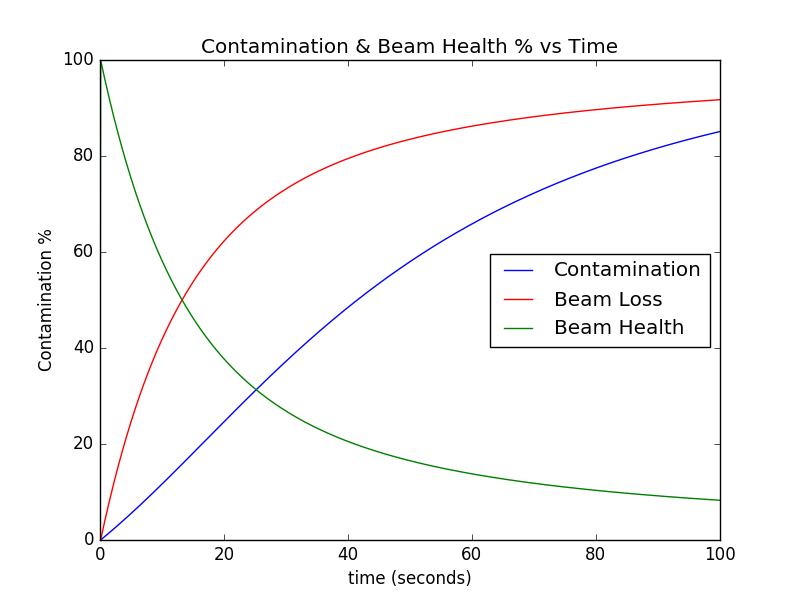
\includegraphics[width=0.5\linewidth]{./Images/Figures/figure_1-4}

A nicely formatted plot with a legend using the matplotlib package.
\begin{lstlisting}
import matplotlib as plt    # Imports the correct packages for plotting.

fig = plt.figure(dpi=1200)  # Increase resolution of the plot.
plt.scatter(x, y, s=0.1)    # Plot x data vs y data with a dot size of 0.1.
fig.suptitle(title, fontsize=12) # adds a title to the figure.

plt.xlabel("x axis label")  # Creates a x-axis label.
plt.ylabel("y axis label")  # Creates a y-axis label.

manage = plt.get_current_fig_manager()
manage.full_screen_toggle() # Makes the plt full screen.

plt.show()                  # Displays plot.
plt.savefig("fileName.png") # Saves the figure as an image
\end{lstlisting}















\section{Pytest \index{Pytest}}

\idx{Pytest} is a powerful and popular testing framework for Python that simplifies the process of writing and executing tests. It offers a straightforward syntax and extensive features for writing test cases, including assertions, fixtures, parameterization, and test discovery. Pytest provides robust support for testing different types of applications, including web applications, APIs, and command-line utilities. It promotes efficient testing practices by emphasizing readability, scalability, and flexibility, making it a preferred choice for many Python developers.

\myindent To run a python test file using pytest, you can call pytest directly via a terminal.
\begin{lstlisting}
pytest -vv test_my_module.py
\end{lstlisting}

To write tests for a function, you must import that function and write a test for it. The \idx{assert} is a basic test keyword is used to check if a statement is true of false.
\begin{lstlisting}
# Code implementation in a Python file (e.g., my_module.py)

def add(x, y):
    """Function to add two numbers."""
    return x + y
\end{lstlisting}

\begin{lstlisting}
# Test case using Pytest (e.g., test_my_module.py)

import pytest
import my_module

def test_add():
    """Test case for the add function."""

    # Test with positive integers
    assert my_module.add(2, 3) == 5
    
    # Test with negative integers
    assert my_module.add(-2, -3) == -5
    
    # Test with zero
    assert my_module.add(0, 0) == 0
    
    # Test with one positive and one negative integer
    assert my_module.add(5, -3) == 2
\end{lstlisting}

